
\subsection{PERM algorithm}
We want now to report an application of the PERM algorithm \cite{PERM}.
We've tried to improve the 2D simulations from the article by increasing the number of iterations (the original was $10^5$ for all proteins).
The first protein for which we've improved the result is $HH(P)^5HH(P)^3H(P)^3HP$, that has a length of 18 amino acids (see Fig. \ref{fig:18_1}).
In particular, we've found $(1.25 \pm 0.35) \times 10^8$ folds with an energy minimum of -4, equal to the benchmark's one.
\begin{figure}[H]
    \centering
    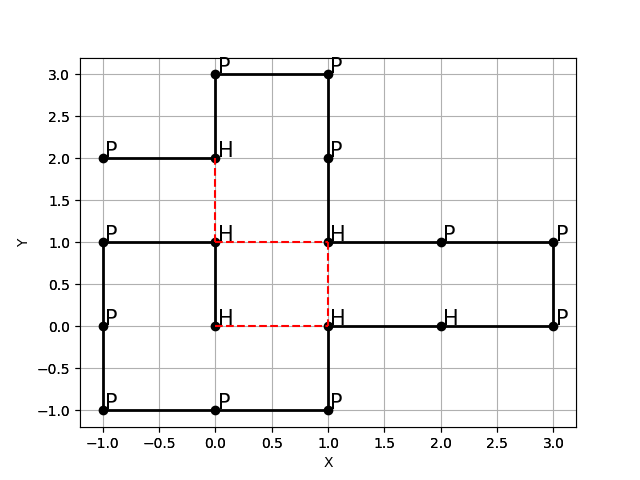
\includegraphics[width=.75\textwidth]{./img/18_1.png}
    \caption{The protein $HH(P)^5HH(P)^3H(P)^3HP$ has reached its energy minimum at -4 after $5 \times 10^6$ iterations.}
    \label{fig:18_1}
\end{figure}

Lastly, we've improved the result is $HHHP(PH)^3PP(HP)^3PH$, that has a length of 20 amino acids (see Fig. \ref{fig:18_1}).
In particular, we've found $(8.900 \pm 0.003) \times 10^10$ folds with an energy minimum of -9, one unit more then the benchmark's one.
\begin{figure}[H]
    \centering
    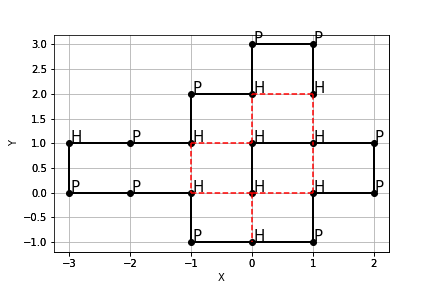
\includegraphics[width=.75\textwidth]{./img/20_2.png}
    \caption{The protein $HHHP(PH)^3PP(HP)^3PH$ has reached its energy minimum at -9 after $10^7$ iterations.}
    \label{fig:20_2}
\end{figure}